\documentclass{article}
\usepackage[fontsize=14]{fontsize}
\usepackage{fontspec}
\setmainfont{CMU Serif}%{Times New Roman}
\setsansfont{CMU Sans Serif}%{Arial}
\setmonofont{CMU Typewriter Text}%{Consolas}
\defaultfontfeatures{Ligatures={TeX}}
\usepackage[math-style=TeX]{unicode-math}
\pagenumbering{gobble}
\usepackage[english, russian, ukrainian]{babel}
\usepackage[
    a4paper,
    footskip=1cm,
    headsep=0.3cm,
    top=2cm,
    bottom=2cm,
    left=2cm,
    right=2cm
    ]{geometry}


\usepackage{graphicx}
\usepackage{caption}
\usepackage{indentfirst}
\usepackage{wrapstuff}

\begin{document}
\begin{wrapstuff}[type=figure, l, top=4, width=0.47\textwidth]
    \centering
    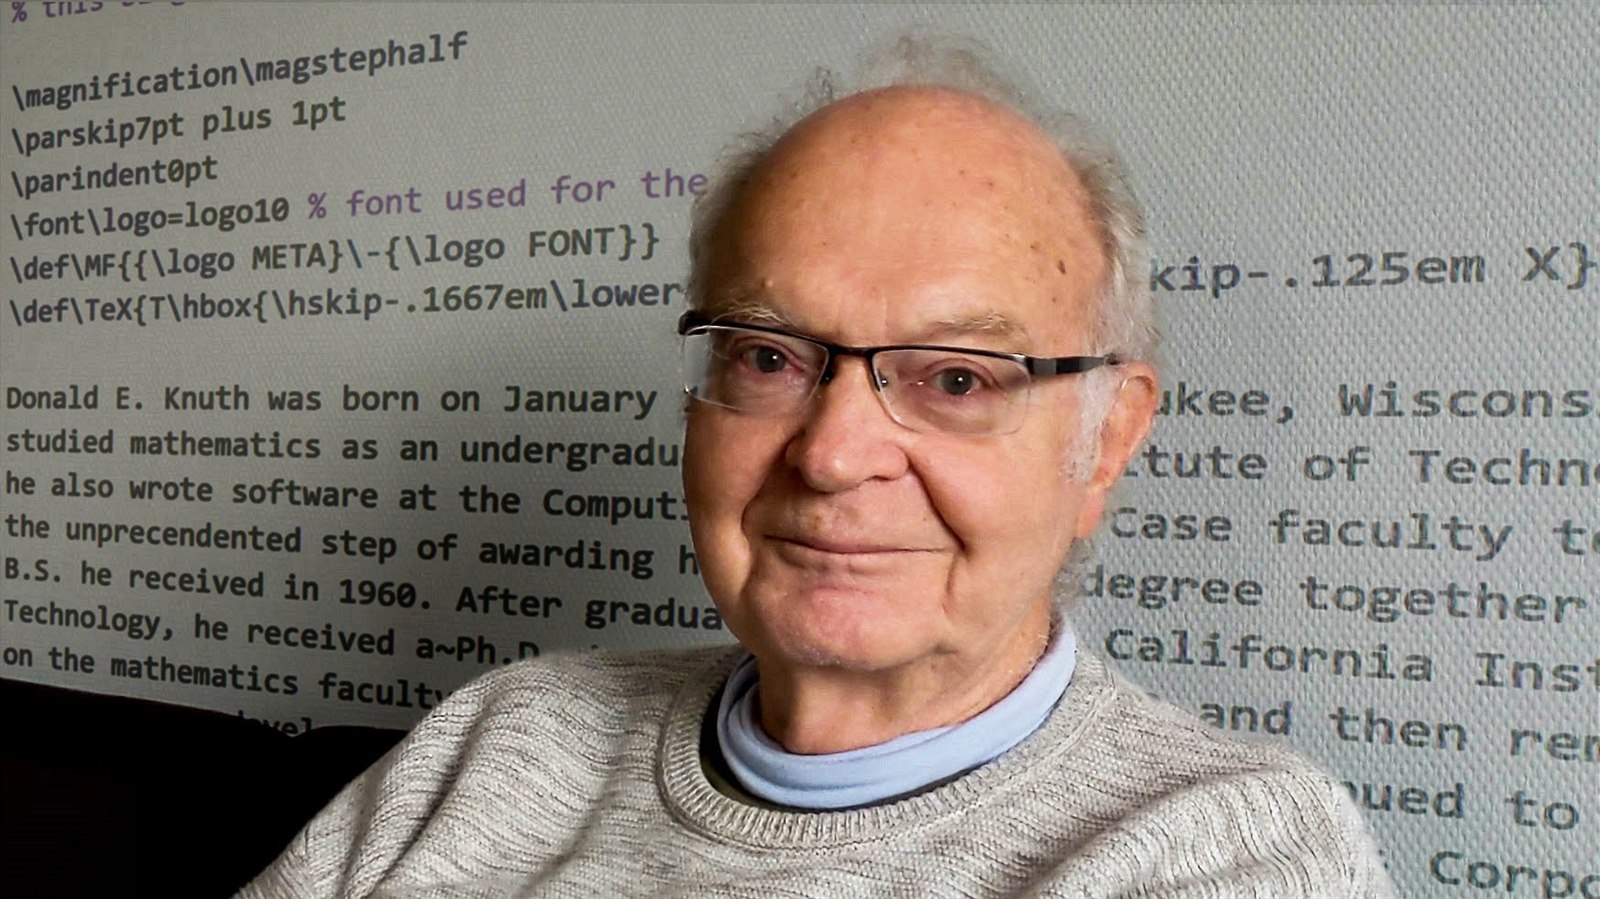
\includegraphics[width=\linewidth]{Knuth.jpeg}
    \caption{Дональд Ервін Кнут}
    \label{fig:knuth}
\end{wrapstuff}
Дональд Ервін Кнут (рис. \ref{fig:knuth}) (10 січня 1938 , Мілвокі, Вісконсин ) --- інформатик, ідеолог програмування та почесний професор Стенфордського університету. Автор фундаментальної праці \textit{«Мистецтво програмування»}; вважається одним з батьків аналізу складності алгоритмів. Розробник типографічної системи \TeX{} та пов'язаної мови визначення шрифтів і системи їх рендерингу \texttt{METAFONT}.

Кнут народився у місті Мілвокі, штат Вісконсин, в сім'ї німецьких американців Генрі Кнута та Луізи Марії Бонінг. Батько Дональда працював на двох роботах: викладав бухгалетерію у Старшій Школі Мілвокі та вів невелике підприємство по друку. Молодший Кнут, навчаючись у тій же школі, отримав багато академічних відзнак, більшість з яких за геніальні способи вирішення різноманітних проблем. Наприклад, у восьмому класі він взяв участь у змаганні, в якому потрібно було відшукати всі слова, які можна скласти з букв словосполуки «Ziegler's Giant Bar». У суддейському списку було 2500 слів, та Дональду вдалось знайти 4500 та перемогти у конкурсі.

Освіта У 1956 році Кнут отримав запрошення до Технологічного Інституту (рис. \ref{fig:cwru}) у Клівленді, Огайо, де вперше познайомився з \texttt{IBM 650}, одним із перших мейнфреймів. Прочитавши посібник до комп'ютера, Кнут вирішив переписати код компілятора для комп'ютера з його колишньої школи, тому що
він вірив, що зможе зробити його краще.

\begin{figure}[ht]
    \centering
    \begin{minipage}{0.5\textwidth}
        \centering
        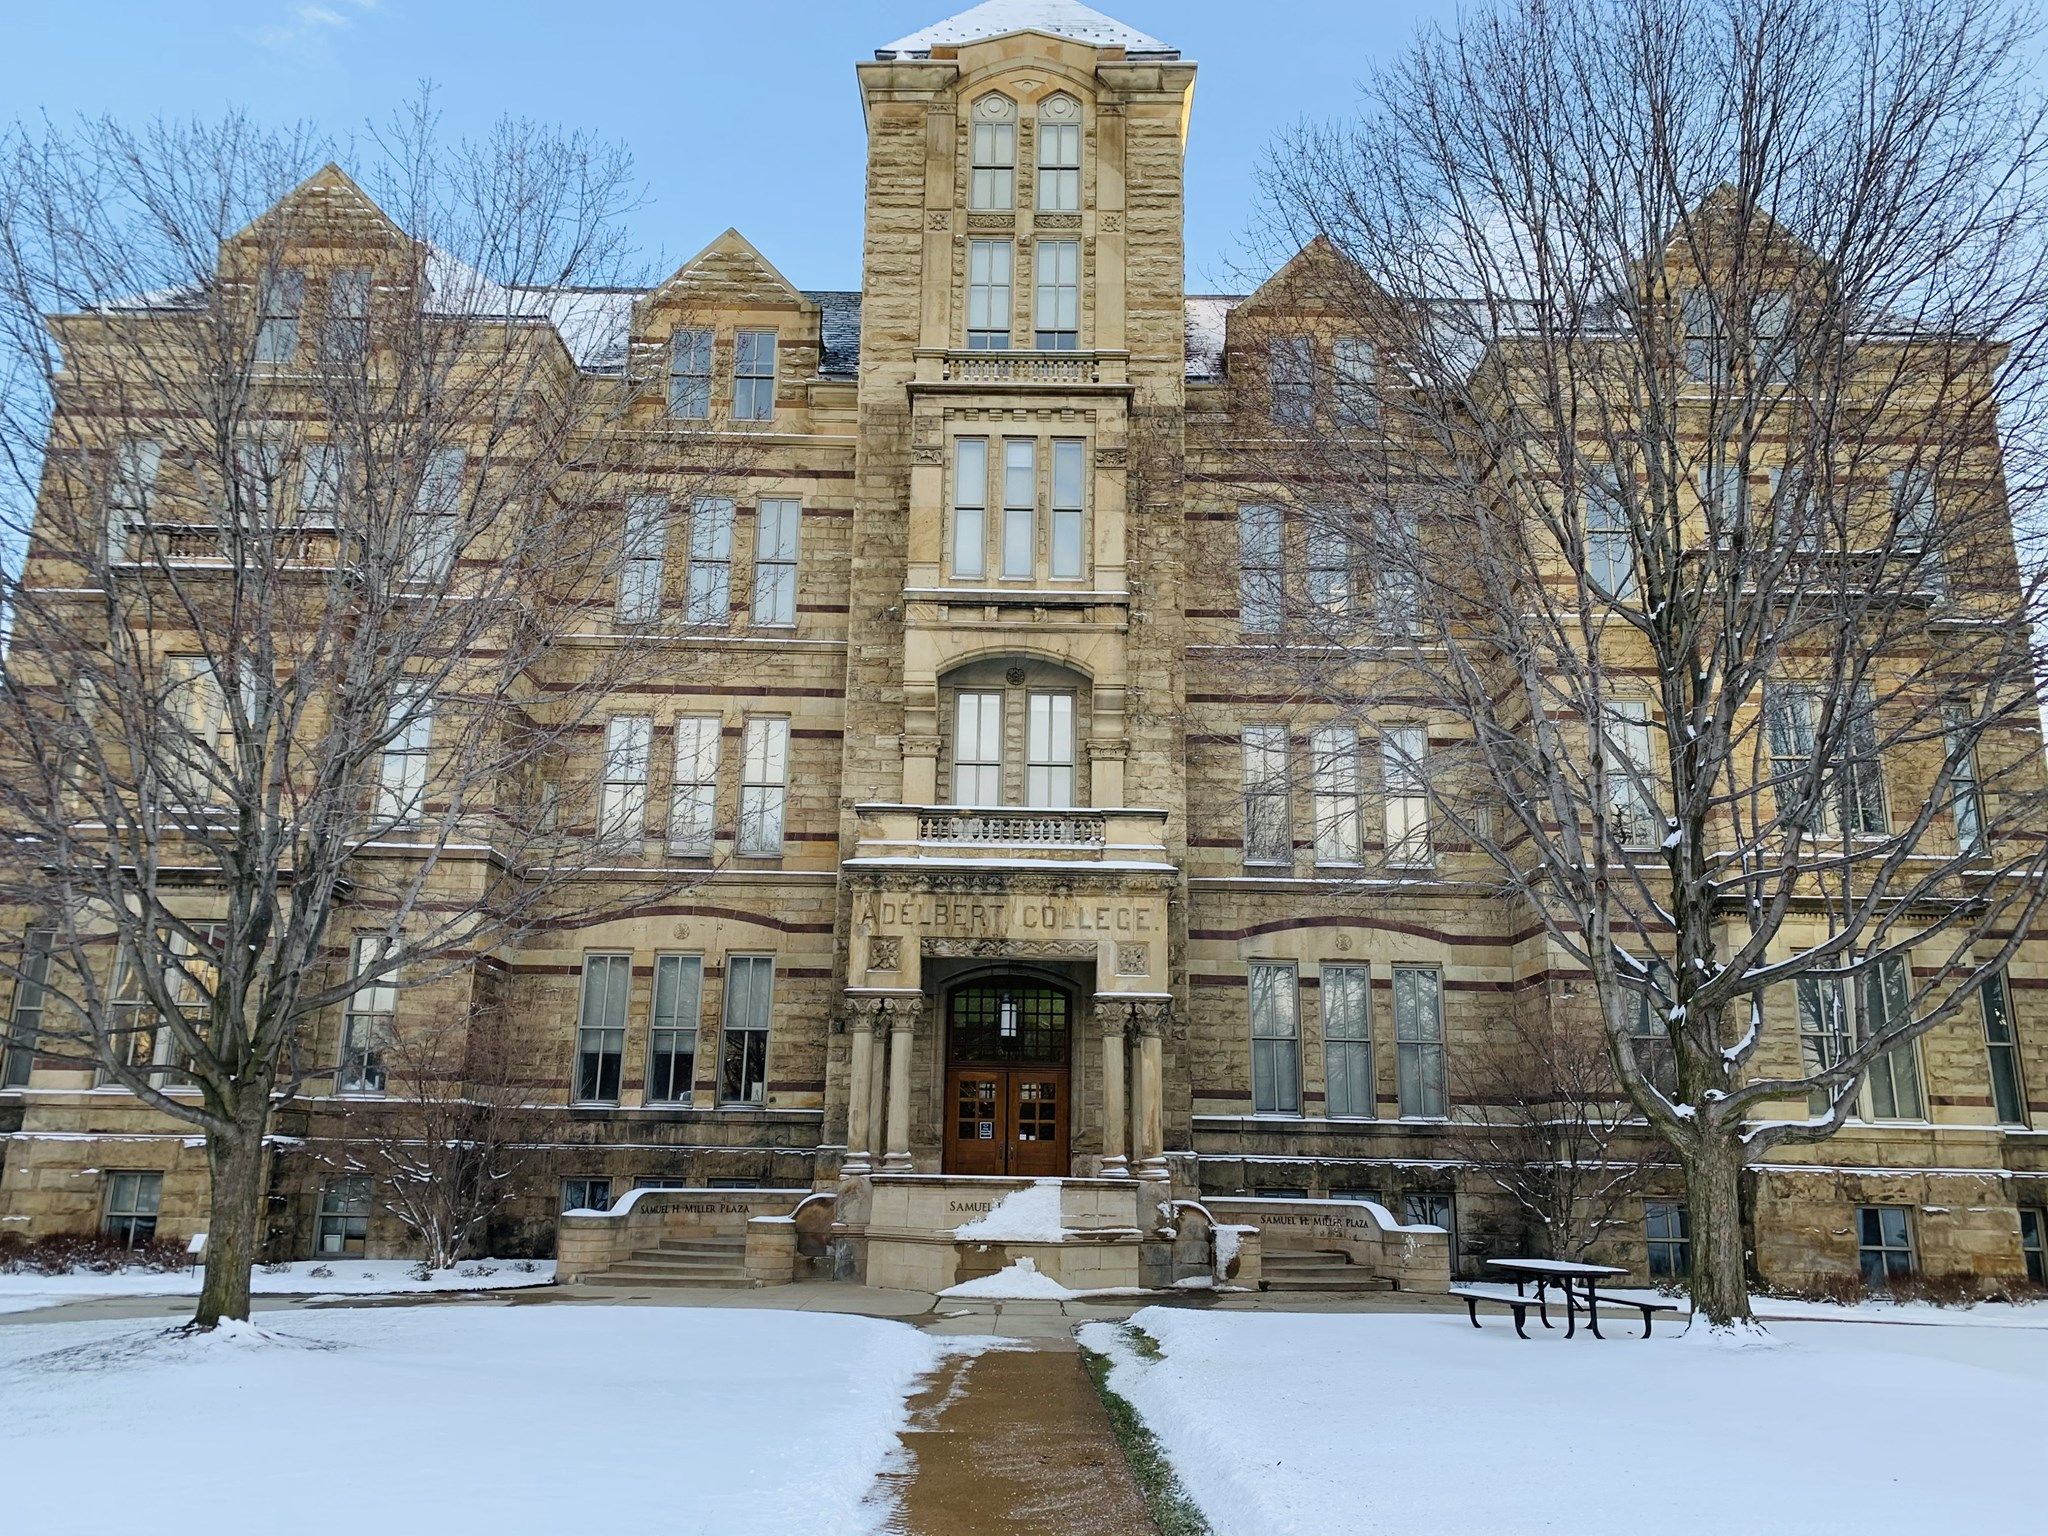
\includegraphics[width=\linewidth]{CWRU.jpg}
    \end{minipage}
    \hspace{0.5cm}
    \begin{minipage}{0.4\textwidth}
        \raggedright 
        \caption{Західний резервний університет Кейса (CWRU)}
        \label{fig:cwru}
    \end{minipage}
\end{figure}

У 1958 році Кнут створив програму, щоб допомогти шкільній баскетбольній команді вигравати більше матчів. Він призначив кожному гравцю «вартість», щоб оцінити імовірність кожного баскетболіста здобути очки. Цей підхід оцінили видання Newsweek і CBS Evening News, згадавши Кнута у своїх випусках.

\end{document}
